\documentclass{article}

%% Page Margins %%
\usepackage{geometry}
\geometry{
    top = 0.75in,
    bottom = 0.75in,
    right = 0.75in,
    left = 0.75in,
}

\usepackage{amsmath}
\usepackage{graphicx}
\usepackage{parskip}

\title{Project Report: Milestone 1 and 2}

\author{Janssen Myer Rambaud (1008107004), Felix Zhang (1007650212)}

\begin{document}
\maketitle

\section{Part I: Planning and Configuration}

\begin{enumerate}
\item \textbf{Breakout Bitmap Display and Memory Map Plan}: 
Our plan is to have a 512 pixel (wdith) x 256 pixel (height) display while keeping the same base address 0x10008000 (\$gp). 
We also plan on having unit widths be 4 pixels x 4 pixels because it remains even while being a better size than say 2 x 2, which is too small.
A table of our memory map plan is given below.
\begin{table}[ht!]
\begin{tabular}{|l|l|l|}
\hline
Data Segment     & Address                                                           & Variable Names           \\ \hline
IMMUTABLE DATA   &                                                                   &                \\ \hline
                 & 0x10008000 (Address of Bitmap Display)                            & ADDR\_DSPL    \\ \hline
                 & 0xffff0000 (Address of Keyboard)                                  & ADDR\_KBRD     \\ \hline
                 & Takes in 1 address (Display width divided by unit width [in pixels])           & SCREEN\_WIDTH  \\ \hline
                 & Takes in 2 addresses for (length, height) of the paddle                                           & PADDLE\_DIM    \\ \hline
                 & Takes in 1 address for width of wall                                           & WALL\_WIDTH    \\ \hline
                 & Takes in 2 addresses (left wall x-coordinate, right wall x-coordinate)                                 & WALLS\_X     \\ \hline
                                  & Takes in 1 address for (height) of buffer                                                           & BUFFER\_HEIGHT \\ \hline
                 & Takes in 1 address buffer colour (used for drawing walls, bricks)              & BUFFER\_COLOUR \\ \hline
                                  & Takes in 1 address for the y coordinate of a brick                & BRICKS\_Y      \\ \hline
                 & Takes in 2 addresses (2-D array that stores colour)               & BRICKS         \\ \hline
                 & Takes in 2 addresses (width, height) for a brick               & BRICKS\_DIM         \\ \hline
                 & Takes in 7 addresses (1 for array length, 6 for elements/colours) & COLOURS        \\ \hline
MUTABLE DATA     &                                                                   &                \\ \hline
                                  & Takes in 1 address for colour of paddle (gray)                                 & PADDLE\_COLOUR \\ \hline
                 & Takes in 1 address for colour of ball (white)                                  & BALL\_COLOUR   \\ \hline
                 & Takes in 2 addresses (x, y) coordinates                           & PADDLE\_COORDS \\ \hline
                 & Takes in 2 addresses (x, y) coordinates                           & BALL\_COORDS   \\ \hline
                 & Takes in 1 address for the movement direction of the ball         & DIRECTION      \\ \hline
\end{tabular}
\end{table}

\item Translate your plan into the .data section of your breakout.asm program. Assemble your program in MARS and inspect memory to ensure it matches your plan. Include a screenshot (or multiple screenshots) of memory demonstrating that it has been laid out according to your plan.

\begin{figure}[ht!]
    \centering
    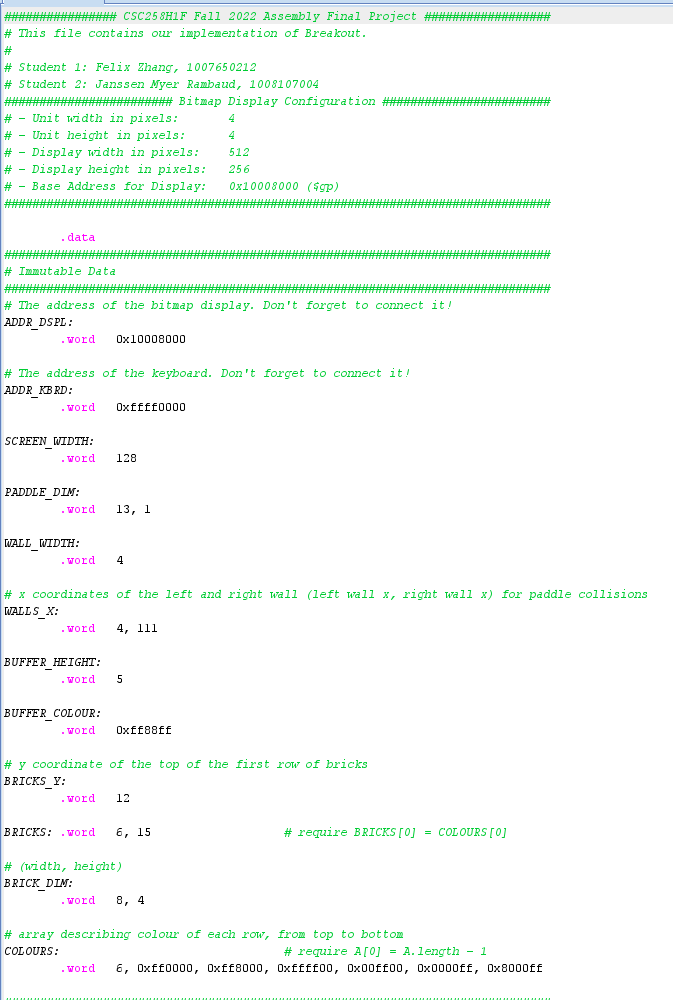
\includegraphics[width=0.5\textwidth]{memory2.png}
    \caption{Screenshot of immutable variables in the .data code section.}
    \label{f:part1_memory1}
\end{figure}

\begin{figure}[ht!]
    \centering
    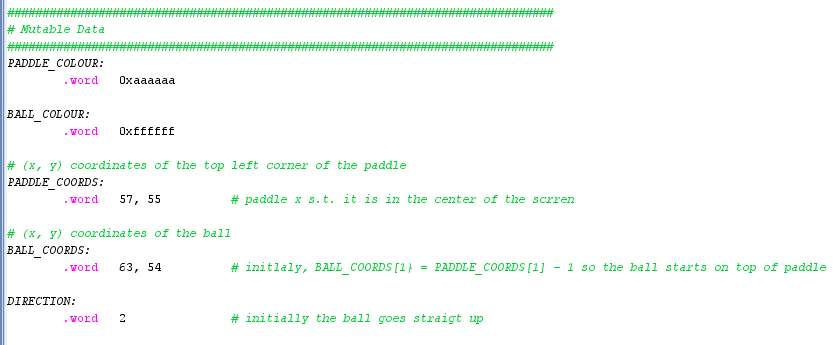
\includegraphics[width=0.5\textwidth]{memory3.png}
    \caption{Second screenshot of mutable variables in the .data code section.}
    \label{f:part1_memory2}
\end{figure}

\begin{figure}[ht!]
    \centering
    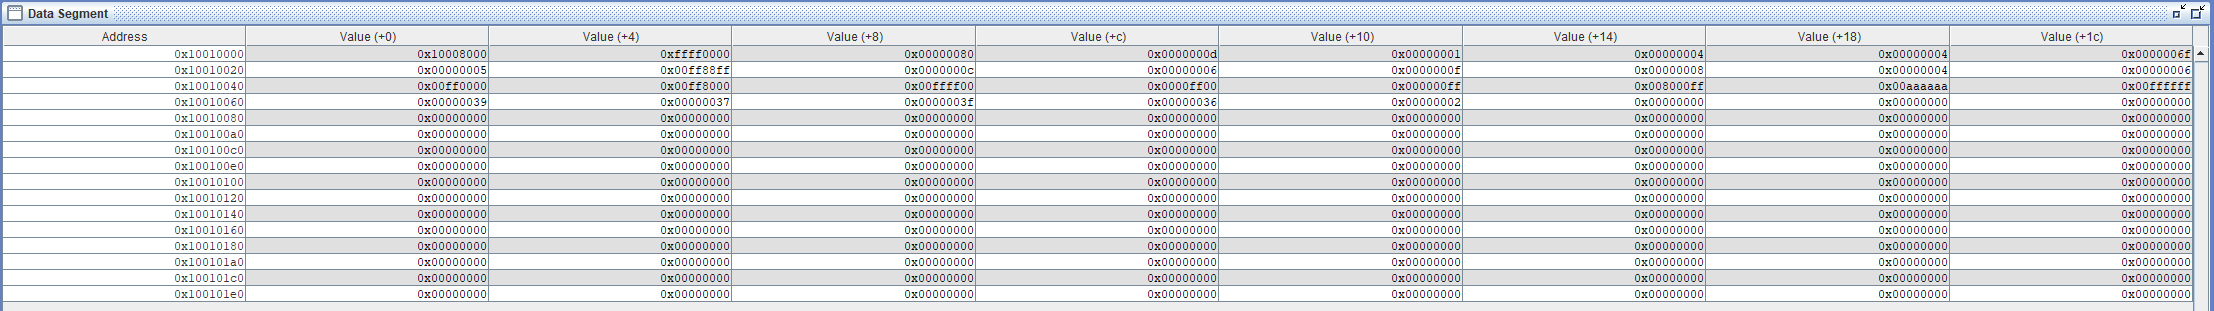
\includegraphics[width=\textwidth]{memory1.png}
    \caption{Screenshot of .data memory.}
    \label{f:part1_memory3}
\end{figure}

\clearpage
\section{Part II: Milestone 1}

\item Draw the scene (Milestone 1)

\begin{figure}[ht!]
    \centering
    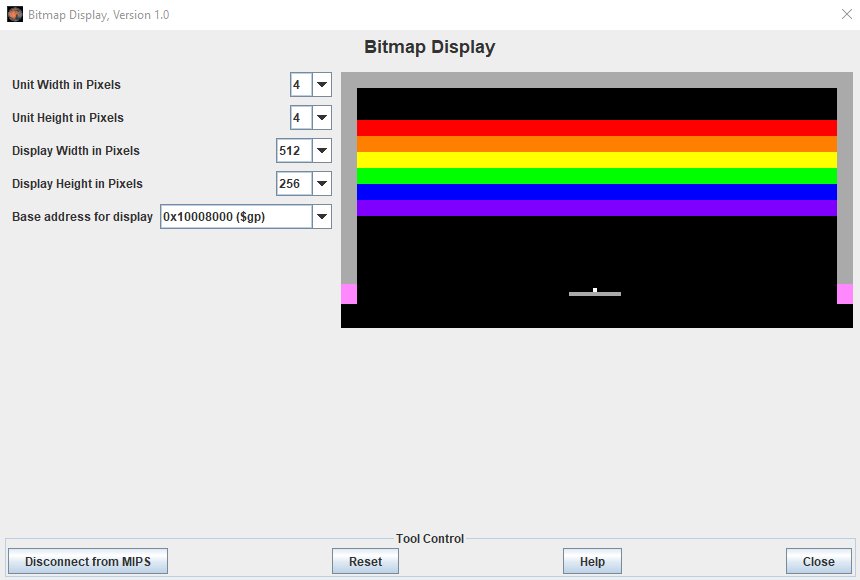
\includegraphics[width=0.8\textwidth]{milestone1_drawing.png}
    \caption{The static scene of Milestone 1 Drawing.}
    \label{f:milestone1_drawing}
\end{figure}

\end{enumerate}

\section{Part III: Milestone 2}

\item \textbf{QUESTION: } How will the ball change directions when it collides? \\[0.4em]
The rules governing how the ball changes directions when it collides are as follows. \\[0.4em]
If it collided with the paddle, then the resulting direction depends on which section of the paddle it hit.
Hitting the leftmost third results it travelling north-east (at a $45^\circ$ angle), the middle third results it travelling north, and the rightmost third results in it travelling north-west (at a $45^\circ$ angle). \\[0.4em]
Otherwise, if it collided with a non-paddle object then the resulting direction depends on the original direction.
If the original direction of ball forms the angle $\theta$ with the surface it collided with, 
then the resulting direction is the reflection of the original direction across the line perpendicular to the collision surface away from the collision point.
For example, if the ball is travelling north-west (at a $45^\circ$ angle) and collides with the left wall, then it begins travelling in the north-east direction (at a $45^\circ$ angle).
Note this also means if the ball was travelling perpendicular to surface with which it collided, then after the collision, it is moving in the reverse direction.
So, if the ball was travelling north before colliding with the bottom of a brick, then it is travelling south after the collision.
\item Upload breakout.asm to MarkUs so that you have a snapshot of your progress so far.

\section{Part IV: Milestone 3}
\item Upload breakout.asm to MarkUs so that you have a snapshot of your progress so far.

\newpage
\section{Part V: DEMONSTRATION 2 Milestone 4 and 5}
\item For our Milestones 4 and 5, we decided to do (a cumulative) 3 easy features and 2 hard features. \\
We chose the easy features: 1 (multiple lives), 5 (pause game), and 9 (launch ball)
and hard features: 1 (track score) and 3 (bricks need multiple hits).
\\ \\
\textbf{Detailed Changes Made: }
\begin{enumerate}
  \item (EASY) 1 - Multiple Lives: There are three hearts at the top left corner which correspond to the amount of lives you have. You start with three lives and once you lose all your hearts (lives), then the game ends. If you "lose" and still have lives left, then you will restart from the initial position where you will have to launch the ball again to CONTINUE playing with the same amount of bricks broken as before.
  \item (EASY) 5 - Pause Game: This is a simple feature where any time the user clicks the exact key 'p', then the game will enter a 'paused' state where there is no movement (from player or game). In order to continue playing, the user must hit any other key, other than 'p', in order for the game to resume playing state and the ball will once again move.
  \item (EASY) 9 - Launch Ball: At the beginning of every game, or at the beginning of every "new life" when the player has been initialized at the starting position (ball and paddle are in the middle of the screen), then they must launch the ball by pressing the spacebar in order to start the game.
  \item (HARD) 1 - Track Score: For every brick hit by the ball, the score on the top right of the screen will increment by 1. In correlation to Multi-Hit Bricks, a 'brighter' coloured brick, once fully broken, awards the player 2 points. After a 'brighter' brick is hit by the ball, it's broken into a 'darker' brick [+ 1 points], and once that 'darker' brick is hit by the ball, it is completely destroyed [+ 1 points].
  \item (HARD) 3 - Multi-Hit Bricks: There are 6 different colours of bricks in this game. There are red, green, and blue coloured bricks as well as their 'darker' counterparts. When the brick is 'brighter' it means that it requires two hits to break. When a 'brighter' brick is hit once, it turns into a 'darker' brick of that same colour. Once a 'darker' brick is broken, then it is deleted/destroyed from the game. 
\end{enumerate}

\newpage
\section{Part VI: HOW TO PLAY}

\textbf{GAME LAYOUT}:
\begin{itemize}
    \item Once you assemble and run the program, you will be met with the game screen as well as the 'STATS' section on the top of the game which contains your lives (hearts) as well as your score in numbers.
\end{itemize}

\begin{figure}[ht!]
    \centering
    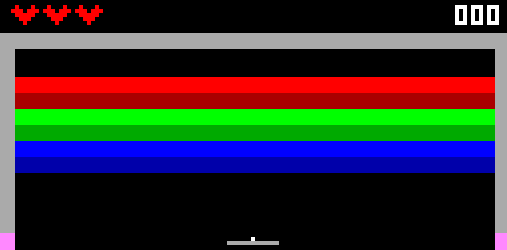
\includegraphics[width=0.5\textwidth]{game_start.png}
    \caption{This is the Game's Initial Start Screen}
    \label{f:Initial Start Screen}
\end{figure}

\textbf{START GUIDE}:
\begin{itemize}
    \item You begin with 3 lives represented by hearts (top-left of screen). 
    \item In this game you will be chasing after the ball (white square) with your paddle (grey rectangle) and attempt to continue bouncing it off the paddle to aim and destroy the coloured blocks above you.
    \item To begin you must launch the ball from the paddle using the [Spacebar].
    \item Your paddle can move left and right using keys [a] for left and [d] for right, but CANNOT go past the walls OR go up and down, this is your paddle's boundary.
    \item The ball can go anywhere within the grey boundary, but if the ball reaches the bottom of the screen, which is past the paddle, then you lose a life.
    \item If you reach this bottom of the screen and lose a life, it will be reflected on the top left of your screen and you will lose a heart as well. If you have remaining lives, then you will restart from the middle of the screen just like when you first started the game. \\ Note: You will continue your progress and the amount of bricks broken, as well as your score, will not be reset.
    \item There are two types of bricks, 'brighter' bricks and 'darker' bricks. For each hit on either brick, you will receive 1 point, which will be reflected in your score on the top-right of the screen. Once hit, a 'brighter' brick will be broken down (transformed) into a 'darker' brick. Once a 'darker' brick is hit, then that brick is 'destroyed' and will turn into empty space that the ball can move through. 
    \item The game ends when you have broken every single brick leaving you with an empty space to freely practice your paddle skills with the ball.
\end{itemize}

\begin{figure}[ht!]
    \centering
    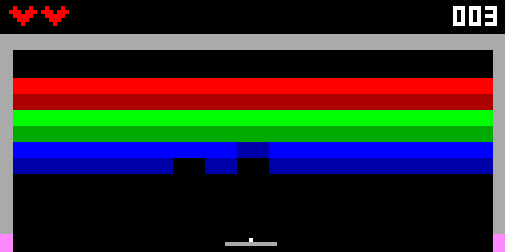
\includegraphics[width=0.5\textwidth]{gameplay1.png}
    \caption{This is what it looks like if the player broke some blocks then lost a life.}
    \label{f: Gameplay 1}
\end{figure}

\textbf{FEATURES}:
\begin{itemize}
    \item Score: Increments by 1 for every block broken. 
    \item Lives: 3 chances to complete the game, every time the ball touches the bottom of the screen, you lose a life. Lose all lives and the game ends.
    \item Collision: The paddle will collide with the wall and cannot go past it. The ball will collide with the paddle or wall, bouncing off of it.
    \item Pause Game: You can enter a paused game state pressing the key [p]. Exit pause with any key aside from [p].
    \item End Game: You can exit/terminate the game when you press either of the two keys, [q] or [x]. \\ 
\end{itemize}

\textbf{SUMMARIZED GAME CONTROLS}: \\ \\
    \textit{PADDLE MOVEMENT} 
    \begin{itemize}
        \item [\textbf{a}] Paddle Left
        \item [\textbf{d}] Paddle Right \\
    \end{itemize}

     \textit{LAUNCH BALL}
    \begin{itemize}
        \item [\textbf{spacebar}] Launch Ball at start (Goes Straight Up) \\
    \end{itemize}
    
    \textit{PAUSE/UNPAUSE GAME}
    \begin{itemize}
        \item [\textbf{p}] Press Once to Set The Game into a Paused State
        \item [\textbf{Any Key}] Any Key Aside from [\textbf{p}] will UnPause The Game and Continue the Ball's Movement. \\
    \end{itemize}
    
    \textit{EXIT GAME}
    \begin{itemize}
        \item [\textbf{q}] Press Once to Exit Game
        \item [\textbf{x}] Press Once to Exit Game \\
    \end{itemize}
    
\begin{figure}[ht!]
    \centering
    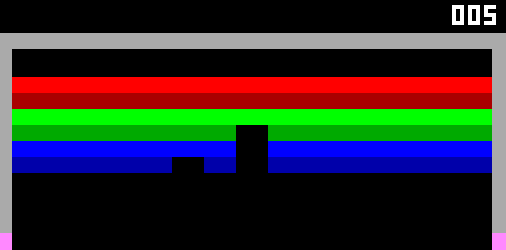
\includegraphics[width=0.5\textwidth]{gameplay2.png}
    \caption{Game Over! The player lost all their lives and the game is finished. This is their final score.}
    \label{f: Gameplay 2}
\end{figure}



\end{document}